In this chapter we will go through the basic setup of the organization, how we work in the project as well as how we communicate within our project. 

\subsection{Roles}
After the applications for different roles were handed in to the project group, the members of the project decided who was going to be appointed to what specific role. Some of the roles applied for was decided not necessary for this type of project, which is why those applicants were assigned different roles. In the end, the company succeeded to appoint people to all the important positions in the company. 

\begin{figure}[hbt!]
\centering
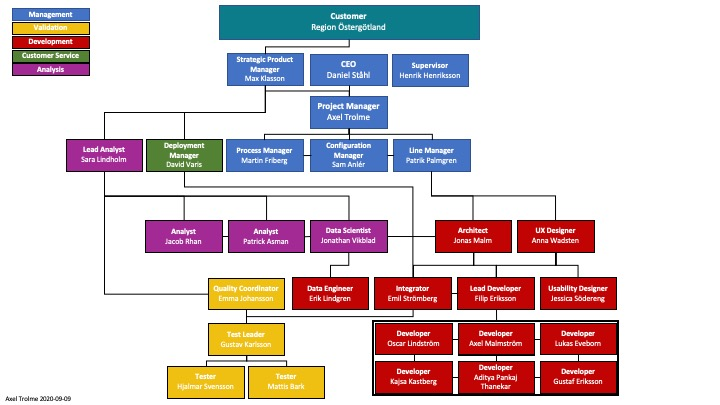
\includegraphics[width=\linewidth]{company_structure}
\caption{A diagram showing the major ways of communication as well as what department the different members of company belongs to}
\label{fig:company structure}
\end{figure}



\subsection{Knowledge/skill}
The company management sent out a form to all the members of the company where the members were supposed to fill in what knowledge they have from before and what knowledge they are currently lacking. In this way, management is able to locate in what areas the skill and knowledge is high and in what areas we are lacking skill and knowledge. The mapping makes it easier for the architect and the lead developer to choose the right tools for the group to work with in order to develop a successful project. If tools are chosen were the group is lacking skill and knowledge, management and the group leaders will easily notice this and can set up a plan on how to increase the knowledge within these areas. 


\begin{figure}[h]
\begin{subfigure}{0.5\textwidth}
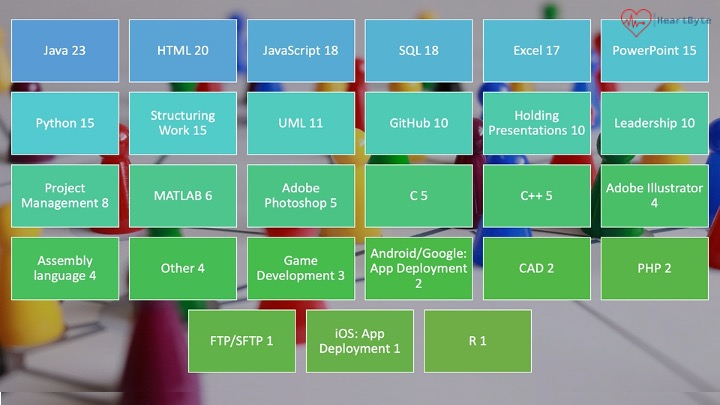
\includegraphics[width=0.9\linewidth, height=5cm]{Pictures/Skills.jpeg} 
\caption{Skills and knowledge that currently exists within the company}
\label{fig:skills}
\end{subfigure}
\begin{subfigure}{0.5\textwidth}
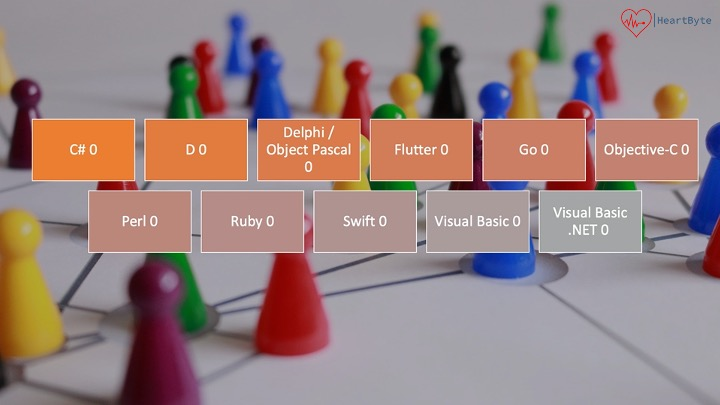
\includegraphics[width=0.9\linewidth, height=5cm]{Pictures/Unskills.jpeg}
\caption{Skills and knowledge that the company currently lacks}
\label{fig:unskills}
\end{subfigure}
\end{figure}


\subsection{Training}
\subsubsection{Workshops}
When development methods include new tools, we select someone responsible for the area who is supposed to gain a deeper understanding about the forementioned tool. The person mentioned is then in charge of making sure that the rest of the team that is supposed to work with the tool gains the required knowledge about it. This is done via workshops online where the responsible person goes through the basics of the tool.  A workshop could also include different brainstorming activities, where the participants are to come up with ideas regarding risks, company name, requirements for the system or tools to use for a specific system. 

\subsubsection{Presentations}
The management produces presentations to give during CEO meetings to educate the team in what has been done during the week and what is to be done during the upcoming weeks. The management is also supposed to highlight what in the process that is the most critical to get done as soon as possible. The presentations might also be used to educate the team in processes and tools that makes the work more effective. Example of tools that this may include is GitLab, Azure DevOps and different programming languages. The presentations could also be about how to handle documents and where to place documents for them to be easily found once they are needed. 

\subsubsection{Resource sharing}
Through sharing resources in Teams and GitLab the team tries to share the knowledge and progression within their work. This assures that the whole team gets to take part of each other’s knowledge and where they currently are in terms of progression. It also prevents two people doing the same thing on different ends. 

\subsection{Communication and reports}
\subsubsection{Group meetings and Discussions}
The team is divided into different teams, both smaller cross-functional teams and teams where the whole group is working together on a specific task. The cross-functional teams makes it easier to share the information between the research and development department and the product and sales department and at the same time making sure that the information is shared and spread across the whole company. These group meetings are supposed to take place at least once every week.  

\subsubsection{Communication directives}
Through set up communication directives every person in the group should know who their main contact is for sharing the information that they want to spread or to gain the information that they want to acquire. A Communication structure has been set in order to make sure that a single person in the entire company talks with everyone else in the company since this can make the information that we are trying to be spread, get lost or be misinterpreted.   

\subsubsection{Reports}
In order to keep the investors, CEO and the customer satisfied and up to date with what is going on in the project, the team will announce weekly status reports. The status reports contains what the group has done during the last week, what is most crucial to be done during the upcoming week as well as what time each project member has put down into the project. This can also help the CEO keep track of the time spent in the project in order to not exceed the budget. 
